\documentclass[tikz,border=5pt]{standalone}
\usetikzlibrary{arrows.meta,positioning,fit}
\begin{document}
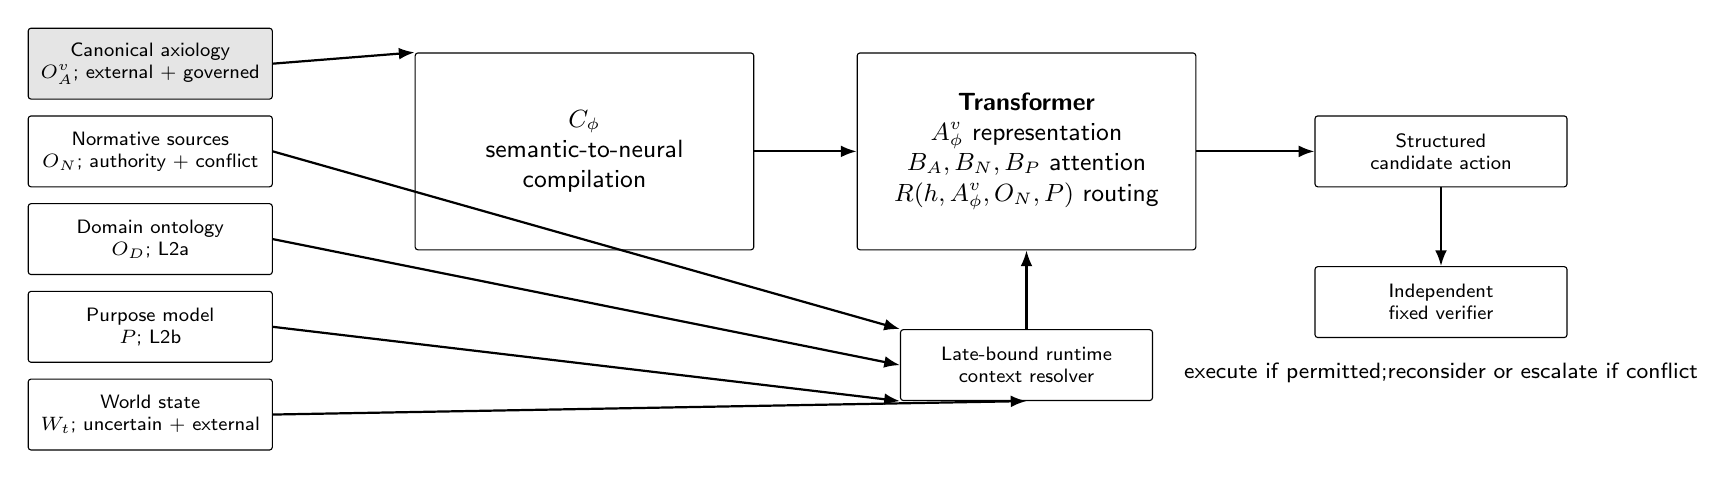
\begin{tikzpicture}[
  source/.style={draw, rounded corners=1pt, minimum width=31mm, minimum height=9mm, align=center, font=\sffamily\scriptsize},
  core/.style={draw, rounded corners=1pt, minimum width=43mm, minimum height=25mm, align=center, font=\sffamily\small},
  result/.style={draw, rounded corners=1pt, minimum width=32mm, minimum height=9mm, align=center, font=\sffamily\scriptsize},
  arrow/.style={-{Latex[length=2mm]}, thick}
]
\node[source, fill=black!10] (axiology) {Canonical axiology\\$O_A^v$; external + governed};
\node[source, below=2mm of axiology] (norm) {Normative sources\\$O_N$; authority + conflict};
\node[source, below=2mm of norm] (domain) {Domain ontology\\$O_D$; L2a};
\node[source, below=2mm of domain] (purpose) {Purpose model\\$P$; L2b};
\node[source, below=2mm of purpose] (world) {World state\\$W_t$; uncertain + external};
\node[core, right=18mm of norm] (compiler) {$C_\phi$\\semantic-to-neural\\compilation};
\node[core, right=13mm of compiler] (transformer) {\textbf{Transformer}\\$A_\phi^v$ representation\\$B_A,B_N,B_P$ attention\\$R(h,A_\phi^v,O_N,P)$ routing};
\node[result, right=15mm of transformer] (candidate) {Structured\\candidate action};
\node[result, below=10mm of candidate] (verify) {Independent\\fixed verifier};
\node[result, below=10mm of transformer] (runtime) {Late-bound runtime\\context resolver};
\draw[arrow] (axiology.east) -- (compiler.north west);
\draw[arrow] (compiler.east) -- (transformer.west);
\draw[arrow] (norm.east) -- (runtime.north west);
\draw[arrow] (domain.east) -- (runtime.west);
\draw[arrow] (purpose.east) -- (runtime.south west);
\draw[arrow] (world.east) -- (runtime.south);
\draw[arrow] (runtime.north) -- (transformer.south);
\draw[arrow] (transformer.east) -- (candidate.west);
\draw[arrow] (candidate.south) -- (verify.north);
\node[font=\sffamily\footnotesize, below=2mm of verify] {execute if permitted;\\reconsider or escalate if conflict};
\end{tikzpicture}
\end{document}
